%!TEX root = ../example.tex
\chapter{Arquitectura del Sistema y Analisis de Tecnologias}
% Paquetes necesarios (deben estar en el preámbulo del documento principal)
% \usepackage{tikz}
% \usepackage{listings}
% \usepackage{amsmath}
% \usepackage{array}
% \usepackage{multirow}
% \usepackage{graphicx}

\section{Introducción a la Arquitectura del Sistema}

El sistema de gestión de quejas y denuncias para la Defensoría del Pueblo (DDP) requiere una arquitectura robusta, segura y escalable que pueda manejar información sensible y garantizar la continuidad del servicio. Este capítulo presenta un análisis exhaustivo de las tecnologías seleccionadas, comparando alternativas y justificando cada decisión arquitectónica en función de los requisitos específicos del proyecto.

\section{Arquitectura General del Sistema}

La arquitectura propuesta sigue un modelo de microservicios distribuidos con un frontend en Angular y un backend híbrido que combina Java Spring Boot y Node.js. Esta combinación permite aprovechar las fortalezas de cada tecnología mientras se mantiene la cohesión y la integridad del sistema.

\begin{figure}[h]
\centering
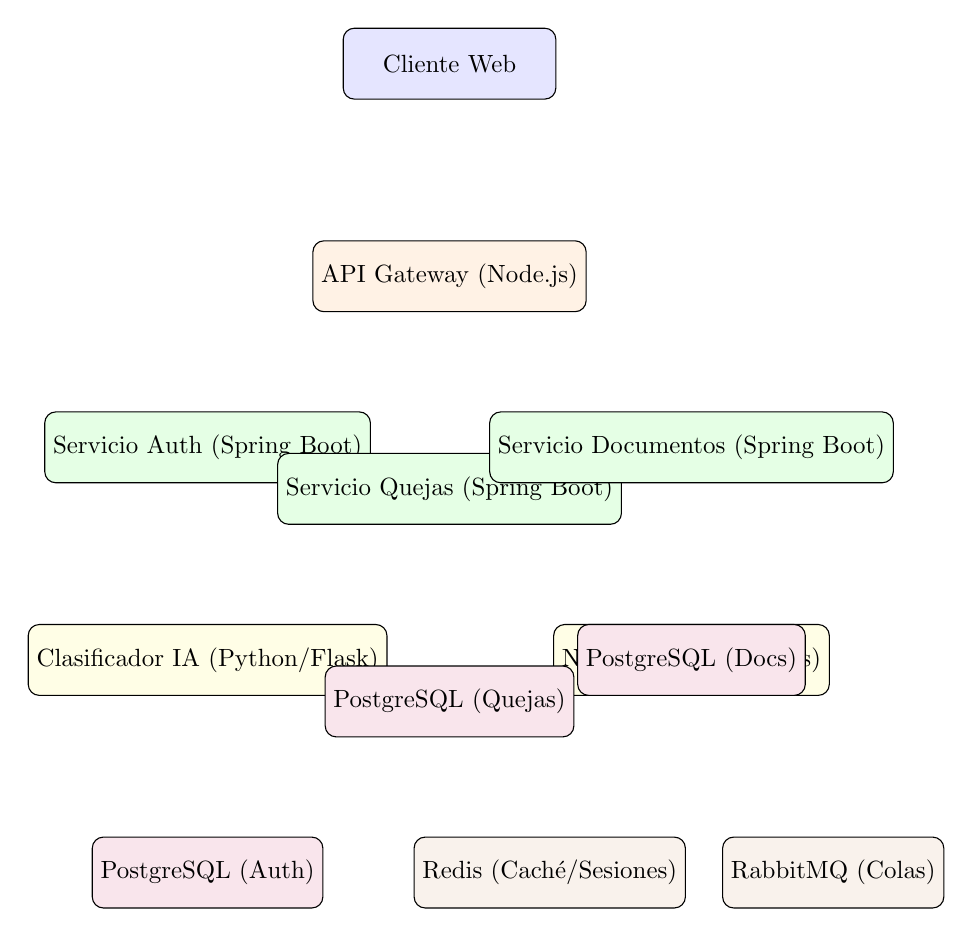
\begin{tikzpicture}[node distance=2cm, scale=0.9, every node/.style={scale=0.9}]
    % Nodos
    \node[draw, rectangle, rounded corners, fill=blue!10, minimum width=3cm, minimum height=1cm] (client) {Cliente Web};
    \node[draw, rectangle, rounded corners, fill=orange!10, minimum width=3cm, minimum height=1cm, below of=client, yshift=-1cm] (gateway) {API Gateway (Node.js)};
    
    \node[draw, rectangle, rounded corners, fill=green!10, minimum width=3cm, minimum height=1cm, below left of=gateway, xshift=-2cm, yshift=-1cm] (auth) {Servicio Auth (Spring Boot)};
    \node[draw, rectangle, rounded corners, fill=green!10, minimum width=3cm, minimum height=1cm, below of=gateway, yshift=-1cm] (quejas) {Servicio Quejas (Spring Boot)};
    \node[draw, rectangle, rounded corners, fill=green!10, minimum width=3cm, minimum height=1cm, below right of=gateway, xshift=2cm, yshift=-1cm] (documentos) {Servicio Documentos (Spring Boot)};
    
    \node[draw, rectangle, rounded corners, fill=yellow!10, minimum width=3cm, minimum height=1cm, below left of=quejas, xshift=-2cm, yshift=-1cm] (ia) {Clasificador IA (Python/Flask)};
    \node[draw, rectangle, rounded corners, fill=yellow!10, minimum width=3cm, minimum height=1cm, below right of=quejas, xshift=2cm, yshift=-1cm] (notif) {Notificaciones (Node.js)};
    
    \node[draw, rectangle, rounded corners, fill=purple!10, minimum width=3cm, minimum height=1cm, below of=ia, yshift=-1cm] (db1) {PostgreSQL (Auth)};
    \node[draw, rectangle, rounded corners, fill=purple!10, minimum width=3cm, minimum height=1cm, below of=quejas, yshift=-1cm] (db2) {PostgreSQL (Quejas)};
    \node[draw, rectangle, rounded corners, fill=purple!10, minimum width=3cm, minimum height=1cm, below of=documentos, yshift=-1cm] (db3) {PostgreSQL (Docs)};
    
    \node[draw, rectangle, rounded corners, fill=brown!10, minimum width=3cm, minimum height=1cm, below of=notif, xshift=-2cm, yshift=-1cm] (redis) {Redis (Caché/Sesiones)};
    \node[draw, rectangle, rounded corners, fill=brown!10, minimum width=3cm, minimum height=1cm, below of=notif, xshift=2cm, yshift=-1cm] (rabbit) {RabbitMQ (Colas)};
    

\end{tikzpicture}
\caption{Diagrama de arquitectura general del sistema DDP}
\label{fig:arquitectura-general}
\end{figure}

\section{Análisis Comparativo de Frameworks Frontend}

El frontend es la cara visible del sistema para los funcionarios de la DDP y los ciudadanos. La selección del framework adecuado es crucial para garantizar una experiencia de usuario fluida, segura y accesible.

\begin{table}[h]
\centering
\caption{Análisis comparativo detallado de frameworks frontend}
\label{tab:comparativa-frontend}
\begin{tabular}{|p{2.5cm}|p{3.5cm}|p{3.5cm}|p{3.5cm}|}
\hline
\textbf{Criterio} & \textbf{Angular} & \textbf{React} & \textbf{Vue.js} \\
\hline
\textbf{Seguridad} & \textbf{Alto}: TypeScript obligatorio, sanitización automática de contenido, protección XSS integrada, soporte nativo para CSP (Content Security Policy) & \textbf{Medio}: JSX puede introducir vulnerabilidades si no se configura adecuadamente, requiere librerías externas para sanitización & \textbf{Medio-Alto}: Plantillas con sanitización automática, pero vulnerabilidades conocidas en versiones anteriores \\
\hline
\textbf{Arquitectura} & \textbf{Opinionada y estructurada}: MVC completo, inyección de dependencias, módulos, componentes, servicios y pipes & \textbf{Basada en componentes}: Libertad total, requiere decisiones arquitectónicas del equipo, propenso a inconsistencias & \textbf{Flexible}: Progresiva, permite múltiples estilos arquitectónicos \\
\hline
\textbf{Curva de aprendizaje} & \textbf{Pronunciada}: TypeScript, RxJS, módulos, inyección de dependencias, conceptos avanzados & \textbf{Moderada}: JSX, hooks, estado, requiere entender conceptos de programación funcional & \textbf{Suave}: HTML templates, opciones API, documentación excelente \\
\hline
\textbf{Mantenibilidad} & \textbf{Excelente}: Estándares compartidos, estructura consistente, inyección de dependencias facilita testing y modularidad & \textbf{Variable}: Depende completamente de decisiones del equipo, puede degenerar en código spaghetti & \textbf{Buena}: Clara separación de concerns, pero puede volverse complejo en aplicaciones grandes \\
\hline
\textbf{Escalabilidad organizacional} & \textbf{Alta}: Diseñado para equipos grandes, lazy loading, módulos feature, workspaces monorepo con Nx & \textbf{Media}: Requiere configuración adicional, herramientas como Next.js o Gatsby para escalar & \textbf{Media-Buena}: Soporte para Composition API mejora organización en proyectos grandes \\
\hline
\textbf{Soporte de pruebas} & \textbf{Nativo}: Karma, Jasmine, TestBed integrados, testing de componentes, servicios y pipes out-of-the-box & \textbf{Requiere configuración}: Jest/React Testing Library, decisiones sobre herramientas de testing & \textbf{Requiere configuración}: Vue Test Utils, Jest/Vitest \\
\hline
\textbf{Ecosistema y estabilidad} & \textbf{Muy estable}: Google, releases semestrales, migración guiada, retrocompatibilidad controlada & \textbf{Estable}: Meta, cambios frecuentes en el ecosistema, fragmentación de librerías & \textbf{Estable}: Comunidad, liderado por Evan You, releases predecibles \\
\hline
\end{tabular}
\end{table}

\subsection{Justificación Detallada de Angular}

Angular se selecciona como el framework frontend principal por las siguientes razones específicas para el contexto de la DDP:

\subsubsection{Seguridad Integrada y Cumplimiento Normativo}

La DDP maneja información sensible de ciudadanos, incluyendo datos personales, denuncias y documentación legal. Angular proporciona características de seguridad críticas:

\begin{itemize}
    \item \textbf{Sanitizacion automatica}: Angular sanitiza automáticamente cualquier valor vinculado al DOM, previniendo ataques XSS (Cross-Site Scripting) sin configuración adicional.
    \item \textbf{TypeScript obligatorio}: El tipado estricto reduce vulnerabilidades relacionadas con tipos dinámicos y facilita el análisis estático de código.
    \item \textbf{Soporte CSP}: Angular funciona nativamente con Content Security Policy, permitiendo políticas restrictivas sin romper funcionalidad.
    \item \textbf{HTTP Interceptors}: Permiten implementar automáticamente tokens CSRF, headers de seguridad y manejo centralizado de errores.
\end{itemize}

\subsubsection{Arquitectura Opinionada para Consistencia Institucional}

En una institución como la DDP, con múltiples equipos de desarrollo y posible rotación de personal, la arquitectura opinionada de Angular garantiza:

\begin{itemize}
    \item \textbf{Estandarización}: Todos los proyectos Angular siguen la misma estructura, facilitando la incorporación de nuevos desarrolladores.
    \item \textbf{Inyección de dependencias}: Sistema nativo que promueve el desacoplamiento y facilita las pruebas unitarias.
    \item \textbf{Módulos funcionales}: Permite organizar el código por dominios de negocio (quejas, usuarios, reportes) con lazy loading para optimizar rendimiento.
    \item \textbf{CLI robusto}: Angular CLI genera código consistente, aplica mejores prácticas y automatiza tareas de build y testing.
\end{itemize}

\section{Análisis Comparativo de Tecnologías Backend}

El backend requiere una combinación de tecnologías que ofrezcan robustez para operaciones críticas y flexibilidad para capas de integración.

\begin{table}[h]
\centering
\caption{Análisis comparativo detallado de tecnologías backend}
\label{tab:comparativa-backend}
\begin{tabular}{|p{2.8cm}|p{4cm}|p{4cm}|}
\hline
\textbf{Criterio} & \textbf{Java Spring Boot} & \textbf{Node.js} \\
\hline
\textbf{Seguridad} & \textbf{Muy alto}: Spring Security, autenticación JWT/OAuth2, autorización basada en roles, protección CSRF, CORS configurable, auditoría integrada & \textbf{Alto}: Helmet.js, express-rate-limit, bcrypt, JWT, pero requiere configuración explícita de cada capa de seguridad \\
\hline
\textbf{Rendimiento} & \textbf{Excelente para operaciones complejas}: Multi-threading, ideal para operaciones transaccionales y computación intensiva & \textbf{Excelente para I/O}: Modelo asíncrono no bloqueante, ideal para APIs REST simples y tiempo real \\
\hline
\textbf{Escalabilidad} & \textbf{Alta}: Soporte nativo para microservicios con Spring Cloud, service discovery (Eureka), configuración distribuida & \textbf{Alta}: Cluster module, PM2, arquitectura orientada a eventos, fácil escalado horizontal \\
\hline
\textbf{Madurez} & \textbf{Muy alta}: 20+ años en entornos empresariales, utilizado por gobiernos y bancos & \textbf{Alta}: 10+ años, ampliamente adoptado pero menos probado en entornos gubernamentales \\
\hline
\textbf{Transaccionalidad} & \textbf{Soporte completo}: @Transactional, gestión declarativa de transacciones & \textbf{Limitado}: No tiene transacciones nativas, requiere manejo manual \\
\hline
\end{tabular}
\end{table}

\subsection{Justificación Detallada de Spring Boot para Microservicios Core}

Spring Boot se selecciona para los microservicios que manejan operaciones críticas de negocio:

\subsubsection{Seguridad a Nivel Empresarial}

\begin{itemize}
    \item \textbf{Spring Security}: Framework completo para autenticación y autorización, con soporte para múltiples proveedores (LDAP, OAuth2, JWT).
    \item \textbf{RBAC granular}: Implementación precisa de roles de la DDP: Abogado Asesor, Subdefensor, Titular, Administrador, etc.
    \item \textbf{Auditoría}: Spring Data Envers permite auditoría completa de cambios en entidades, crucial para trazabilidad legal.
\end{itemize}

\subsubsection{Integridad Transaccional}

Los procesos de la DDP requieren garantías transaccionales:

\begin{itemize}
    \item \textbf{Transacciones ACID}: Garantía de consistencia en operaciones que involucran múltiples entidades.
    \item \textbf{Aislamiento}: Niveles de aislamiento configurables para evitar lecturas sucias.
    \item \textbf{Compensación}: Patrones SAGA implementables con Spring Boot para transacciones distribuidas.
\end{itemize}

\subsection{Justificación Detallada de Node.js para Capas de Integración}

Node.js complementa la arquitectura en roles específicos:

\subsubsection{API Gateway}

\begin{itemize}
    \item \textbf{Alto rendimiento I/O}: Maneja miles de conexiones concurrentes con bajo consumo de recursos.
    \item \textbf{Proxy inverso}: Express/Fastify como proxy para enrutar peticiones a microservicios.
    \item \textbf{Rate limiting}: Implementación eficiente de límites de peticiones.
\end{itemize}

\subsubsection{Servicio de Notificaciones}

\begin{itemize}
    \item \textbf{Tiempo real}: Socket.io para notificaciones en tiempo real a funcionarios.
    \item \textbf{Email/SMS}: Nodemailer, Twilio, librerías maduras para comunicación multicanal.
    \item \textbf{WebSockets}: Manejo eficiente de conexiones persistentes.
\end{itemize}

\section{Análisis del Sistema de Base de Datos}

La selección del motor de base de datos es crítica para garantizar integridad, seguridad y rendimiento.

\begin{table}[h]
\centering
\caption{Análisis exhaustivo de PostgreSQL para el proyecto DDP}
\label{tab:postgresql-analisis}
\begin{tabular}{|p{3.5cm}|p{4.5cm}|p{4cm}|}
\hline
\textbf{Aspecto} & \textbf{Ventajas} & \textbf{Consideraciones} \\
\hline
\textbf{Seguridad} & 
\begin{minipage}[t]{4.5cm}
\begin{itemize}
    \item Cumplimiento ACID estricto
    \item Cifrado nativo (SSL/TLS)
    \item Roles y permisos granulares
    \item Row-Level Security (RLS)
\end{itemize}
\end{minipage} & 
Requiere configuración adecuada de permisos \\
\hline
\textbf{Integridad de datos} & 
\begin{minipage}[t]{4.5cm}
\begin{itemize}
    \item Foreign keys, constraints
    \item Transacciones ACID
    \item Triggers y reglas
\end{itemize}
\end{minipage} & 
Modelo relacional estricto \\
\hline
\textbf{Madurez} & 
\begin{minipage}[t]{4.5cm}
\begin{itemize}
    \item 30+ años de desarrollo
    \item Comunidad global masiva
    \item Documentación extensa
\end{itemize}
\end{minipage} & - \\
\hline
\textbf{Rendimiento} & 
\begin{minipage}[t]{4.5cm}
\begin{itemize}
    \item Optimizador de consultas avanzado
    \item Índices múltiples
    \item Particionamiento nativo
\end{itemize}
\end{minipage} & 
Requiere tuning: VACUUM, índices \\
\hline
\end{tabular}
\end{table}

\subsection{Justificación Detallada de PostgreSQL}

\subsubsection{Integridad de Datos Jurídicos}

La información manejada por la DDP (quejas, denuncias, expedientes) requiere garantías absolutas de integridad:

\begin{itemize}
    \item \textbf{Transacciones atómicas}: Las operaciones que involucran múltiples tablas se ejecutan completamente o no se ejecutan.
    \item \textbf{Integridad referencial}: Las foreign keys garantizan que no existan huérfanos.
    \item \textbf{Check constraints}: Validaciones de negocio a nivel base de datos.
\end{itemize}

\subsubsection{Seguridad a Nivel de Fila (RLS)}

PostgreSQL permite implementar políticas de seguridad a nivel de fila, crucial para los roles de la DDP:

\section{Análisis Comparativo de Arquitecturas: Microservicios vs Monolito}

La decisión arquitectónica fundamental define cómo evolucionará el sistema.

\begin{table}[h]
\centering
\caption{Comparativa detallada: Microservicios vs Arquitectura Monolítica}
\label{tab:comparativa-arquitectura}
\begin{tabular}{|p{3cm}|p{4.5cm}|p{4.5cm}|}
\hline
\textbf{Criterio} & \textbf{Microservicios} & \textbf{Monolito} \\
\hline
\textbf{Escalabilidad} & 
\begin{minipage}[t]{4.5cm}
\begin{itemize}
    \item Independiente por servicio
    \item Escalado horizontal granular
\end{itemize}
\end{minipage} & 
\begin{minipage}[t]{4.5cm}
\begin{itemize}
    \item Escalado completo
    \item Desperdicio de recursos
\end{itemize}
\end{minipage} \\
\hline
\textbf{Mantenibilidad} & 
\begin{minipage}[t]{4.5cm}
\begin{itemize}
    \item Código modular por dominio
    \item Despliegue independiente
\end{itemize}
\end{minipage} & 
\begin{minipage}[t]{4.5cm}
\begin{itemize}
    \item Código acoplado
    \item Cambios afectan toda la aplicación
\end{itemize}
\end{minipage} \\
\hline
\textbf{Seguridad} & 
\begin{minipage}[t]{4.5cm}
\begin{itemize}
    \item Aislable por servicio
    \item Menor superficie de ataque
\end{itemize}
\end{minipage} & 
\begin{minipage}[t]{4.5cm}
\begin{itemize}
    \item Centralizada
    \item Mayor superficie de ataque
\end{itemize}
\end{minipage} \\
\hline
\textbf{Tolerancia a fallos} & 
\begin{minipage}[t]{4.5cm}
\begin{itemize}
    \item Circuit breakers
    \item Aislamiento de fallos
\end{itemize}
\end{minipage} & 
\begin{minipage}[t]{4.5cm}
\begin{itemize}
    \item Fallo total
    \item Sin aislamiento
\end{itemize}
\end{minipage} \\
\hline
\end{tabular}
\end{table}

\subsection{Justificación Detallada de Microservicios para la DDP}

\subsubsection{Separación por Dominios Funcionales}

La DDP tiene dominios claramente diferenciados:

\begin{enumerate}
    \item \textbf{Servicio de Gestión de Quejas}: Core del sistema, maneja el ciclo de vida completo de quejas y denuncias.
    \item \textbf{Servicio de Autenticación y Autorización}: Gestiona usuarios, roles y permisos.
    \item \textbf{Servicio de Documentos}: Almacena y gestiona archivos adjuntos.
    \item \textbf{Servicio de Notificaciones}: Envía alertas por email, SMS, notificaciones push.
    \item \textbf{Clasificador IA}: Procesa quejas entrantes para clasificarlas automáticamente.
\end{enumerate}

\subsubsection{Patrones de Resiliencia Implementados}

\begin{lstlisting}[language=Java, caption=Ejemplo de Circuit Breaker con Resilience4j]
@CircuitBreaker(name = "clasificadorIA", fallbackMethod = "clasificarFallback")
public Clasificacion clasificarQueja(Queja queja) {
    return clasificadorClient.clasificar(queja);
}

public Clasificacion clasificarFallback(Queja queja, Exception ex) {
    log.warn("Clasificador IA no disponible, usando clasificacion por defecto", ex);
    return new Clasificacion("PENDIENTE", "GENERAL");
}
\end{lstlisting}

\subsection{API Gateway como Punto Único de Entrada}

El API Gateway (Node.js) proporciona:

\begin{itemize}
    \item \textbf{Autenticación centralizada}: Verifica tokens JWT antes de enrutar.
    \item \textbf{Rate limiting}: Previene abusos y ataques DoS.
    \item \textbf{Enrutamiento inteligente}: Dirige peticiones al servicio correspondiente.
    \item \textbf{Aggregación}: Combina respuestas de múltiples servicios.
    \item \textbf{Logging y monitoreo}: Registro centralizado de todas las peticiones.
\end{itemize}

\section{Matriz de Selección Tecnológica y Evaluación de Riesgos}

\begin{table}[h]
\centering
\caption{Matriz de selección tecnológica con ponderación por criterios}
\label{tab:matriz-seleccion}
\begin{tabular}{|p{2.5cm}|c|c|c|c|c|c|}
\hline
\textbf{Tecnología} & \textbf{Seguridad (30\%)} & \textbf{Escalabilidad (20\%)} & \textbf{Mantenibilidad (20\%)} & \textbf{Curva aprendizaje (10\%)} & \textbf{Estabilidad (20\%)} & \textbf{Puntuación ponderada} \\
\hline
Angular & 5 (1.5) & 4 (0.8) & 5 (1.0) & 3 (0.3) & 5 (1.0) & \textbf{4.6} \\
\hline
React & 3 (0.9) & 4 (0.8) & 3 (0.6) & 4 (0.4) & 4 (0.8) & \textbf{3.5} \\
\hline
Vue.js & 4 (1.2) & 4 (0.8) & 4 (0.8) & 5 (0.5) & 4 (0.8) & \textbf{4.1} \\
\hline
Spring Boot & 5 (1.5) & 5 (1.0) & 5 (1.0) & 3 (0.3) & 5 (1.0) & \textbf{4.8} \\
\hline
Node.js & 4 (1.2) & 5 (1.0) & 4 (0.8) & 4 (0.4) & 4 (0.8) & \textbf{4.2} \\
\hline
PostgreSQL & 5 (1.5) & 4 (0.8) & 4 (0.8) & 3 (0.3) & 5 (1.0) & \textbf{4.4} \\
\hline
Microservicios & 4 (1.2) & 5 (1.0) & 5 (1.0) & 2 (0.2) & 4 (0.8) & \textbf{4.2} \\
\hline
Monolito & 4 (1.2) & 3 (0.6) & 3 (0.6) & 4 (0.4) & 4 (0.8) & \textbf{3.6} \\
\hline
\end{tabular}
\end{table}

\subsection{Análisis de Riesgos Tecnológicos}

\begin{table}[h]
\centering
\caption{Matriz de riesgos tecnológicos y mitigaciones}
\label{tab:riesgos}
\begin{tabular}{|p{3.5cm}|p{4cm}|p{4cm}|}
\hline
\textbf{Riesgo} & \textbf{Impacto} & \textbf{Mitigación} \\
\hline
\textbf{Complejidad de microservicios} & Alto & Service mesh, opentelemetry para trazabilidad \\
\hline
\textbf{Seguridad en Node.js} & Medio & SCA (Snyk/npm audit), actualización automática \\
\hline
\textbf{Rendimiento de PostgreSQL} & Medio & Monitoreo con pg\_stat\_statements, índices adecuados \\
\hline
\textbf{Obsolescencia tecnológica} & Bajo & Versiones LTS, contenerización \\
\hline
\textbf{Brecha de conocimiento} & Medio & Programa de capacitación, consultoría inicial \\
\hline
\end{tabular}
\end{table}

\section{Conclusiones de la Selección Tecnológica}

La combinación tecnológica seleccionada para el sistema de la DDP responde a las necesidades específicas de una institución pública que maneja información sensible y requiere:

\begin{itemize}
    \item \textbf{Seguridad}: Angular y Spring Boot proporcionan características de seguridad maduras y probadas.
    \item \textbf{Escalabilidad}: Microservicios permiten crecimiento independiente por dominio funcional.
    \item \textbf{Mantenibilidad}: La arquitectura modular y las tecnologías opinionadas garantizan consistencia.
    \item \textbf{Integridad de datos}: PostgreSQL asegura cumplimiento ACID y trazabilidad legal.
    \item \textbf{Flexibilidad}: Node.js complementa para casos donde su modelo asíncrono es ventajoso.
\end{itemize}

Esta arquitectura prepara a la DDP para un crecimiento sostenible, adaptándose a futuros requisitos sin comprometer la seguridad ni la integridad de los datos de los ciudadanos.
\end{document}